\chapter{Les données utilisateur}
\section{Initialisation et modification des données de l'utilisateur}
L'initialisation des données de l'utilisateur se fait lors du premier démarrage du logiciel (cf.\ref{fig:renseignementInformationsEntreprise}).

Pour modifier ces informations, il suffit de cliquer sur le bouton \textbf{Paramètres}\index{Barre d'outils!Paramètres} de la barre d'outils \ref{fig:modifierUtilisateur} ou de passer par le menu <<Fichier $\rightarrow$ Paramètres>>. 

\begin{figure}[H]
	\centering
	%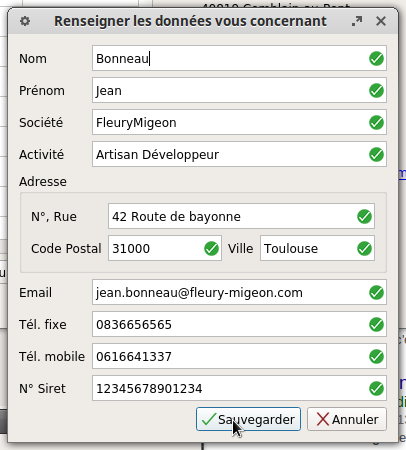
\includegraphics[height=7cm]{screens/modifierUtilisateur.png}
	\caption{Fenêtre de saisie des informations de l'utilisateur}
	\label{fig:modifierUtilisateur}
\end{figure}